\chapter{Implementation}
\label{chp:implementation}
This chapter explains how the hybrid vehicle, which is similar to the Toyota Prius second generation, was modelled in Simulink. Then the implementation details in Matlab of each of the six game-theoretical approaches are described.

\section{Hybrid Vehicle Model}
The model of the hybrid vehicle is split into different controllers and each of them is responsible for controlling the corresponding part of the hybrid. The chapter describes the Drive Cycle Controller, the Power Controller, the Gasoline Engine Controller, the Electric Motor Controller, the Gearbox and the Vehicle dynamics. The game-theoretical logic is included in the Power Controller, which is the principal controller where the solution is computed. It is shown in the next section.

\subsection{Drive Cycles Controller}
This subsection deals with the demand of speed which comes from the Drive Cycle and how it is transformed to acceleration demand, which corresponds to the acceleration pedal in a vehicle.

Two different drive cycles were simulated. The FTP-75 drive cycle is intended to test light-duty vehicles in the U.S. and measure their gas emissions and fuel economy. It lasts for 1874s, the total distance it covers is 17.77km and the average speed is 34.1 km/h. The drive cycle contains three phases - cold start from 0-504s, transient phase from 505-1369s and hot start from 1370-1874. The last phase is exactly the same as the first phase. Figure \ref{fig:ftp75} shows the time and speed of this drive 
cycle.

\begin{figure}[h]
\centering
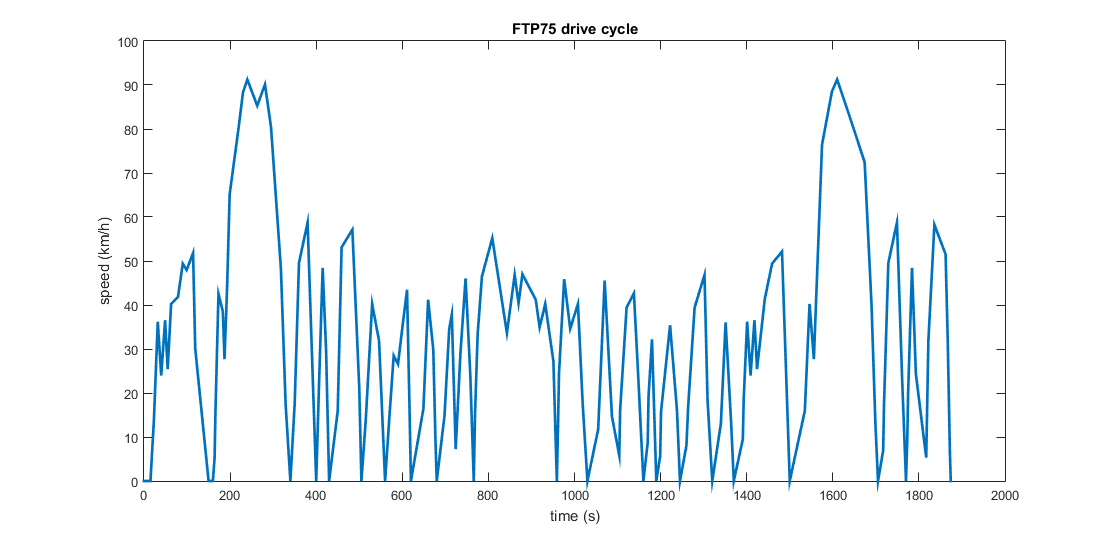
\includegraphics[scale=0.45]{figures/FTP75}
\caption{FTP drive cycle}
\label{fig:ftp75}
\end{figure}

The NEDC drive cycle was invented to test light-duty cars in Europe. Its duration is 1180s, the distance is 11.02km and the average speed 33.6km/h. It contains four equivalent urban driving phases called ECE-15. They last from 0-780s and there is also a fourth highway driving phase called EUDC from 781-1180s. Figure \ref{fig:nedc} shows the time versus the speed in the NEDC drive cycle.

\begin{figure}[h]
\centering
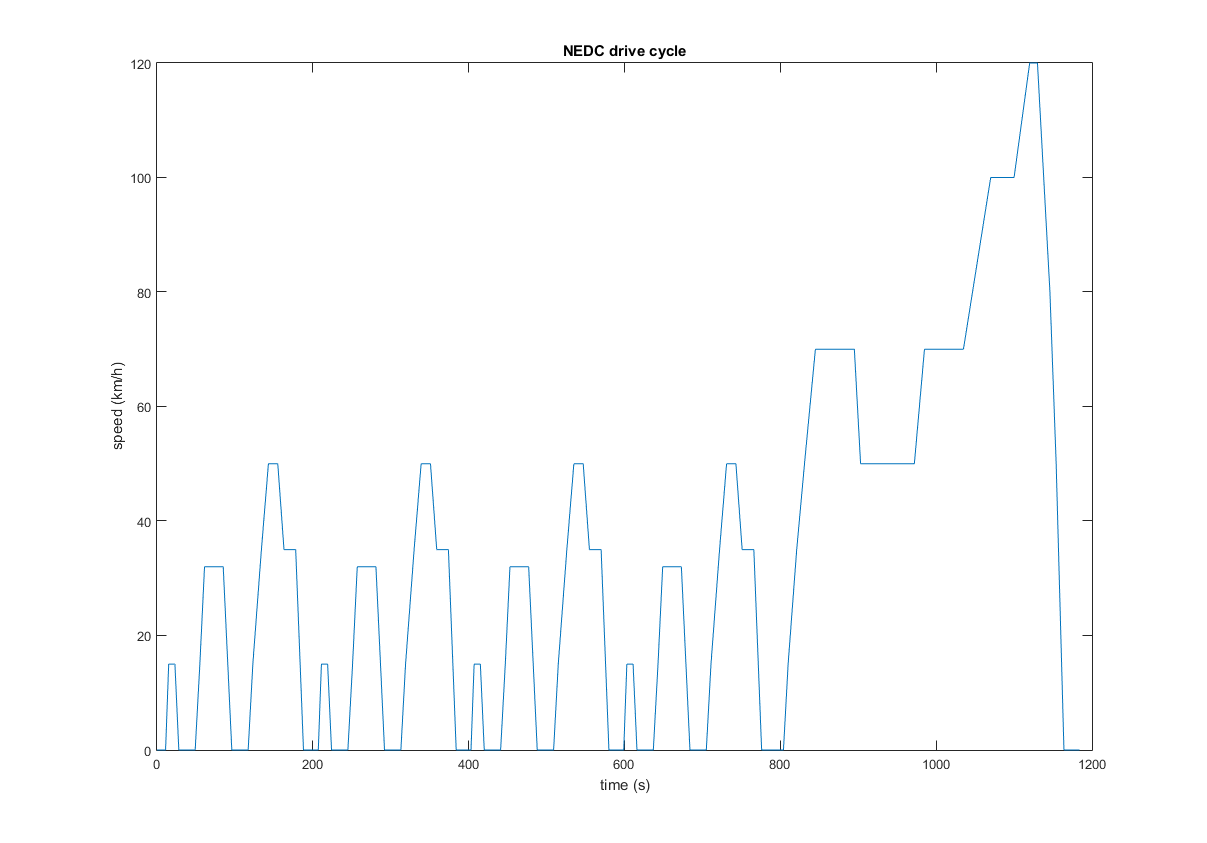
\includegraphics[scale=0.45]{figures/NEDC}
\caption{NEDC drive cycle}
\label{fig:nedc}
\end{figure}

The Speed Control block takes as input the demanded speed from the drive cycle and the actual speed of the vehicle both in \textit{km/h} and calculates as output the acceleration which lies between -1 and 1 where a negative value means braking and a positive value means acceleration. A value of 0 corresponds to cruising or maintaining a constant speed. In order to calculate the acceleration demand, the difference between the demanded and actual speed is taken.

\subsection{Power Controller}
The Power Controller takes as input the acceleration demand $a$ and the state of charge $SOC$ of the battery which comes from the Electric Motor Controller. In order to transform the acceleration demand into torque demand $\tau_{dem}$, the acceleration is scaled by the maximum torque of 400 \textit{Nm} which can be requested. This value was chosen since this is the maximum output torque of the Toyota Prius electric motor. The minimum demanded torque is -400 \textit{Nm} which corresponds to deceleration. The current motor speed $\omega_{mot}$ is mapped to the torque of the motor which it is capable of generating at this moment. This value is taken as upper limit and its negated value is taken as a lower limit of the torque. 

There are two subsystems in the Power Controller, the Battery Management and the Game Theory Controller. The first of them takes as input the battery $SOC$, its current in \textit{A}, its voltage in \textit{V} and computes the required recharge power $P_{batReq}$ and the battery limit $P_{batLim}$. The recharge power is requested when the SOC of the battery lies between 40 and 60\%. If the SOC falls below 40\% then the battery is forced to be recharged even if that means not meeting the drive cycle requirements and not achieving the demanded speed. After the battery has been charged up to 60\%, the recharging stops and the requested battery power is set to 0. The battery limit calculation takes into account that the maximum voltage of the battery is 200V and that its maximum power is 21 kW.

The Game Theory Controller is the primary place where the computation of the solution to the power distribution problem happens. The outputted demanded torque $\tau_{dem}$ is fed into the Game Theory Controller block. In addition, the other inputs of this block are required power, which is:
\begin{equation}
P = \tau \times \omega
\end{equation}
where power $P$ is in \textit{W}, torque $\tau$ is in \textit{Nm} and the velocity $\omega$ is angular \textit{rad/s}.
The Game Theory Controller also receives the battery SOC in \%, the generator $\omega_{gen}$, engine $\omega_{eng}$, motor $\omega_{mot}$ speeds all in \textit{rad/s}, the Total Fuel consumed up to this moment from the beginning of the drive cycle $TF$ in \textit{litres}, the battery limit and the required battery recharge power $P_{batReq}$ as described in the Battery Management subsystem above. The Game Theory Controller block contains the game-theoretical logic embedded as a Matlab function. Apart from it, it also regulates the speed of the engine by taking the difference between the required driving power $P_{drive}$ and the recharge power for the battery $P_{batReq}$. The resulting power is given as an input to a lookup table to find the corresponding engine speed in \textit{rpm}. To obtain the Generator torque $\tau_{gen}$ the engine torque and the generator speed $\omega_{gen}$ in \textit{rad/s} are taken. If the motor needs to provide additional power for the battery, this power is taken to be the sum of the battery available power and the generator power. The battery available power $P_{batAv}$ is computed in a separate subsystem using the engine torque $\tau_{eng}$, speed $\omega_{eng}$ and power $P_{eng}$, battery recharge power $P_{batReq}$ and battery limit $P_{batLim}$. 
Four values come as a result from the Game Theory Controller, the engine throttle $\theta$, the motor torque $\tau_{mot}$, the generator torque $\tau_{gen}$, the reference engine speed in \textit{rpm} $\omega_{eng}$. These are fed to a final Speed Controller block for controlling the engine speed which outputs the final engine throttle $\theta$ as percentage from the maximum possible torque of the engine $\tau_{engMax}$.

\subsection{Engine Controller}
The Engine Controller receives the throttle in \% as input and sends the torque as output. The Gasoline Engine library block implements a gasoline fuel engine and its speed controller. Firstly, the masked library block and then the extensions added to it to will be explained.

In the Gasoline Engine block the input signal between 0 and 1 indirectly controls the engine speed. Whenever the input is outside of the allowed range it is limited to 0 or 1 respectively. The mapping of speed in \textit{rpm} to torque in \textit{Nm} is implemented by a lookup table. The throttle goes through a Switch block which ensures that the maximum speed of the engine is not exceeded. If this happens, the throttle is set to 0. Otherwise the torque and the angular velocity are measured and after that the torque flows to the output. The angular velocity measured in \textit{rad/s} is fed back to the lookup table in \textit{rpm} to find the corresponding torque and it is also given to the switch block for controlling the maximum speed.

An additional functionality which was implemented to extend the library block was to limit the torque from 0 to 136 and also speed from 0 to 6000 rpm. Figure \ref{fig:engineTorqueSpeed} shows the torque speed curve of the engine. It provides maximum torque of 135 to 136 in the speed range 2800 - 3200 rpm. For this reason when the acceleration is constant and the engine provides maximum torque, there is a discrepancy in the simulation results, because the speed keeps jumping from 2800 to 3200 quickly, which is inefficient. Therefore, a hysteresis was implemented by a Relay block which has a switch on and a switch off point values. When the signal lies between 2800 and 3200 rpm it is either set to 2800 or to 3200 rpm to prevent such jittering.

A Driveline environment is connected to the output of the Gasoline Engine block which provides the simulation environment. In addition, attaching a Torsional Spring-Damper \citep{tsdMatlab} allows the torque to flows between two rotating axes, the base and the follower. The input (base) is connected to the output of the Gasoline Engine library block which is the torque, whereas the output (follower) is grounded using an Housing block to prevent it from rotating. The Torsional Spring-Damper takes as parameters the stiffness (spring rate) set to 0 \textit{N*m/rad} and the damping (kinetic friction) set to 0.2079 \textit{N*m*s/rad}. The torque depends on the relative displacement angle and relative angular velocity. Moreover, the outputted torque from the Gasoline Engine block has another connection to an Inertia block, which acts as a rigid rotating body. Torque and angular velocity are measured and given along with the throttle to a Scope block for displaying the results of the engine. Power is also calculated by taking the product of torque and velocity.

A separate subsystem is responsible for the fuel and gas emissions calculations. It receives the engine speed in \textit{rpm} and the torque and outputs Total Fuel $TF$ in \textit{l}, Fuel Consumption $FC$ in \textit{l/100km}, CO emissions, HC emissions, NOX emissions all in \textit{g/km}. In order to calculate them lookup tables are applied, which hold the data for the gas emissions in grams per second \textit{g/s}. To transform \textit{g/s} into \textit{g/km} the total distance travelled is required. That is why the average speed of the drive cycle is calculated and is multiplied with the total time. 

\subsection{Electric Motor Controller}
The Electric Motor Controller is a large subsystem containing the battery, a DC/DC converter, the motor and the generator. It receives as input the demanded motor torque and generator torque. It outputs the battery characteristics and the actual motor torque and actual generator torque.

The battery is modelled by a Battery block of a Nickel-Metal-Hydride type. The nominal voltage is 200V and the rated capacity is 6.5Ah. At the beginning of the simulation the battery is fully charged, its state of charge is set to 100\%. The discharge characteristics are shown in Figure \ref{fig:batteryDischarge}. The first figure shows the nominal discharge current and the second shows the discharge curves at the specific discharge currents. The discharge model $f_1$ and charge model $f_2$ of the battery are \citep{batteryMatlab}:

\begin{equation}
\begin{split}
f_1(it,i*,i,Exp) = E_0 - K \cdot \frac{Q}{Q-it} \cdot i* - K \cdot \frac{Q}{Q-it} \cdot it + Laplace^{-1} \bigg( \frac{Exp(s)}{Sel(s)} \cdot 0 \bigg)
\end{split}
\end{equation}

\begin{equation}
\begin{split}
f_2(it,i*,i,Exp) = E_0 - K \cdot \frac{Q}{|it|+0.1 \cdot Q} \cdot i* - K \cdot \frac{Q}{Q-it} \cdot it + Laplace^{-1} \bigg( \frac{Exp(s)}{Sel(s)} \cdot \frac{1}{s} \bigg)
\end{split}
\end{equation}
where $E_0$ is the constant voltage, $Exp(s)$ is the exponential zone dynamics in $V$, $Sel(s)$ is the battery mode, 0 for discharging and 1 for charging, $K$ is polarization constant in $Ah^{-1}$, $i*$ is the low frequency current dynamics in $A$, $i$ is the battery current in $A$, $it$ is the extracted battery capacity in $Ah$, $Q$ is the maximum battery capacity in $Ah$.

The DC/DC converter is directly attached to the battery. Its purpose is to convert direct current from one voltage to another, from the battery voltage to the motor and generator voltage. The DC bus voltage of the whole electric system is maintained at 500V. 

The Electric Motor subsystem is modelled similar to the AC6 - 100 kW Interior Permanent Magnet Synchronous Motor (PMSM) Drive library model \citep{ac6Matlab}. The motor is a PMSM as in the Toyota Prius. However, the implemented model in this thesis is a 50 kW instead of 100 kW and the bus voltage is 500VDC instead of 288VDC like in the AC6 library model. In total there are four main parts of the electric motor - the PMSM, the Three-phase Inverter, the VECT controller and the Speed Controller. 

The inputs of the Motor block are torque in \textit{Nm}, enable 0 or 1, speed in \textit{rad/s} and the plus and minus from the battery. The outputs are the three motor characteristics - stator current in \textit{A}, rotor speed in \textit{rad/s}, electromagnetic torque in \textit{Nm} and the speed control containing the reference torque in \textit{Nm}. The Speed controller receives as input the speed and an Enable signal. The incoming torque is converted to speed using a lookup table and fed into the Speed controller. It outputs the torque and transmits it to the VECT controller, whose output are three reference line currents. They are given to the Three-phase converter which converts voltage. The Simulink library block Permanent Magnet Synchronous Machine \citep{pmsmMatlab} is used for the implementation of the motor itself. On this motor there are 8 poles and the rotor is of type salient-pole, which means that the magnets are buried. It is a three-phrase motor and has a sinusoidal back electromotive force EMF. The mechanical input can either be the torque \textit{Nm} or the speed in \textit{rad/s}, but in this case it is the speed. Depending on the sign of the torque coming as input the block can either work as a motor or as a generator. When the sign is positive it operates as a motor and if it is negative, it acts as a generator. 

The motor's characteristics are plotted in the Electric Motor scope. These include the current in \textit{A}, the rotor speed \textit{rpm}, the measured and the reference torque \textit{Nm} and also the power in \textit{W}. The outputted torque from the motor is limited between -400 and 400 \textit{Nm} and is also used as output from the whole Electric Motor Controller.

The Generator block is modelled in the exact same manner as the Motor block. Again the Simulink block Permanent Magnet Synchronous Machine \citep{pmsmMatlab} is utilized. Nevertheless, the generator is a 30 kW machine in contrast to the 50 kW motor. The minimum and maximum torque are the same as in the motor, -400 and 400 \textit{Nm} and are limited within this range using a Saturation block. The generator's resulting stator current in \textit{A}, rotor speed in \textit{rpm}, measured and reference torque in \textit{Nm} and power in \textit{W} are displayed in the Generator scope.

\subsection{Transmission}
The main purpose of the transmission or the gearbox is to incorporate the torque from the engine, motor and generator and to transmit the combined torque to the vehicle. In the Toyota Prius this is the Power Split device. 

The Transmission subsystem receives as input the torque from the engine, motor and generators. The output is the combined torque of these three which flows into the Vehicle dynamics subsystem where it is transmitted to the wheels. The transmission consists of a planetary gear with a carrier, ring and sun gears. Each of these three gears is connected to one source of torque. The engine is connected to the planetary carrier, the motor is attached to the ring gear and the generator to the sun gear. After merging the torques they are outputted from the ring, where the motor is attached. While the axle of the carrier and thus rotates the ring and sun gears using the inside planet gears, the ring gear axle transmits the torque to the wheels in the Vehicle model. The sun gear's axle, where the generator is attached, is responsible for converting the power of the engine to electrical energy.

The Planetary gear block itself is implemented by the model in \citet{planetMatlab}. It consists of one planet-planet gear and one ring-planet gear. The parameter ring/sun gear ratio is fixeed and is set to 2.6. When the sun rotates in one direction, the ring co-rotates in the other direction with regard to the carrier gear and vice versa. This gear ratio $g_{RS}$ also corresponds to the number of teeth in the ring and sun gear and to the torque ratio between them $g_{RS} = N_R/N_S = \tau_R/\tau_S$. There are two geometry constraints regarding the radii of the gears. The radius of the carrier is the sum of the radius of the sun and planet gears $r_C = r_S + r_P$, whereas the radius of the ring gear is the sum of the carrier radius and the planet radius $r_R = r_C + r_P$. In addition, there are two kinematic constraints which say that $r_C\omega_C = r_S\omega_S + r_P\omega_P$ and $r_R\omega_R = r_C\omega_C + r_P\omega_P$. This means that the angular velocity of the carrier is the sum of the velocities of the sun and planet gear and the angular velocity of the ring is the sum of the carrier and planet velocities.

In the Transmission subsystem there are three scopes which show simulation results. The first scope is about torque and displays the three torques of the carrier, ring and the sun all in \textit{Nm}. The second scope is the speed scope showing the angular velocity in \textit{rad/s} of the carrier, sun and ring. Lastly, the power scope shows sun, ring and the carrier power in \textit{W} which should be the sum of the ring and sun power.

\subsection{Vehicle dynamics}
The last subsystem models the vehicle dynamics. It receives as input the combined torque which is coming from the motor port, where all three torques of the motor, engine and generator are merged. The torque is measured with a Torque sensor, whose output is connected to a Torsional Spring-Damper. The parameters stiffness and damping are set to 0 \textit{N*m/rad} and 0.1 \textit{N*m*s/rad} respectively. A Simple Gear block \citep{simpleGearMatlab} transfers the torque. The block is a gearbox consisting of two axes, a base and a follower, which rotate with a fixed ratio set to 4.113. Whenever the sign of the two axes is the same, they rotate in the same direction and when it is different, they rotate in opposite directions. An Inertia block with 0.5 $kg*m^2$ is attached to the torque output of the Simple Gear before it goes to the differential. 

The Differential block as in \citet{differentialMatlab} represents a differential gear which has a longitudinal axis as input and two lateral axes as output. Usually the two lateral axes rotate with distinct angular velocities. A single parameter is necessary for the Differential block and that is the  drive gear ratio $g_D$, in this case 1. It predetermines the relationship $\omega_B = \frac{1}{2} \cdot g_D(\omega_{F1} + \omega_{F2})$ between the longitudinal base axis $\omega_B$ and the two lateral axes $\omega_{F1}$ and $\omega_{F2}$. Either of the following two cases can be true. Firstly, the longitudinal shaft is the same as the two lateral shafts when they rotate with the same velocity, $\omega_{F1} = \omega_{F2}$. Secondly, the longitudinal shaft can be locked, $\omega_B = 0$ and the lateral shafts rotate in the opposite direction, $\omega_{F1} = -\omega_{F2}$. The last constraint is that the input and output power of the differential must be the same: $\omega_B \tau_B = \omega_{F1} \tau_{F1} + \omega_{F2} \tau_{F2}$.

Each of the two output shafts of the differential are connected to one inertia with 0.5 $kg*m^2$. The left and right tires are modelled with the Tire block \citep{tireMatlab}. It has the following parameters, effective rolling radius in 0.3 \textit{m}, rated vertical load 3000 \textit{N}, peak longitudinal force at rated load 3500 \textit{N}, slip at peak force at rated load 10\% and relaxation length at rated load 0.2 \textit{m}. The inputs of the Tire block are $V_x$ and $F_z$, where $V_x$ is the wheel longitudinal velocity in \textit{m/s} and $F_z$ is the vertical load in \textit{N}. The outputs are Omega, which is the wheel angular velocity expressed in \textit{rad/s} and $F_x$ is the longitudinal force in \textit{N}. Figure \ref{fig:tire} shows the forces applied to the wheel.

\begin{figure}[h]
\centering
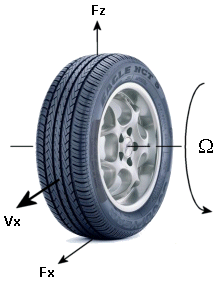
\includegraphics[scale=0.8]{figures/tire}
\caption{Forces affecting the tire \citep{tireMatlab}}
\label{fig:tire}
\end{figure}

Each of the two tires is connected to the primary block in the Vehicle Dynamics subsystem. This is the Longitudinal Vehicle Dynamics \citep{vehicleDynMatlab}, which implements the dynamics of a vehicle with two axles and four wheels. Its inputs are the incline angle $\beta$ and the front and rear longitudinal forces $F_{xf}$ and $F_{xr}$, which come from each of the front and rear tires' outputs $F_x$. The block produces as outputs the vehicle velocity $V_x$ and also the vertical load forces for the front and rear tires $F_{zf}$ and $F_{zr}$. These two are transmitted to the $F_z$ input ports of the wheels. In addition, the block calculates the vehicle velocity which is also fed back to the wheels' ports $V_x$. Before sending the output of the whole Vehicle Dynamics subsystem, the speed is transformed from \textit{m/s} to \textit{km/h}.

\section{Game-theoretical algorithms}
This chapter describes the implementation of all six game-theoretical approaches in Matlab.